\documentclass{article}
\usepackage[utf8]{inputenc}
\usepackage[options ]{algorithm2e}
\usepackage{algorithmic}
\usepackage{algorithm}

\usepackage[english]{babel}
\usepackage[utf8]{inputenc}
\usepackage{amsmath}
\usepackage{amsfonts}
\usepackage{graphicx}
\usepackage[colorinlistoftodos]{todonotes}
\usepackage{algorithm}
\usepackage{algpseudocode}

\title{The Readers Writers problem}
\author{Diaconescu Bogdan-Florin\\ CR 3.2 A, Anul 3}

\usepackage{natbib}
\usepackage{graphicx}

\begin{document}
\maketitle
\newpage
\section{Problem statement}
\hspace{0.5 cm}
There is a shared resource which should be accessed by multiple processes. There are two types of processes in this context. They are reader and writer. Any number of readers can read from the shared resource simultaneously, but only one writer can write to the shared resource. When a writer is writing data to the resource, no other process can access the resource. A writer cannot write to the resource if there are non zero number of readers accessing the resource at that time.

\section{Implementation/Solution}
\hspace{0.5 cm}
I created a class Resource that contains the methods the readers and writers will use to coordinate access to the database. Access is coordinated using semaphores. For writing process I created a function: "void write(int writerNumber)" that has as parameter the writer's number. First, acces to resource and queue is obtained using semaphores: resourceAccess and serviceQueue. If access is obtained, allow other process to acces service queue (serviceQueue.release()). Then the writing begins and at the end release exclusive acces to resource (resourceAccess.release()).

\hspace{0.5 cm}
For reading process, I created a function: "void read(int readerNumber)" that has as parameter the reader's number. It's necessary to obtain access to the queue and the readCount variable using serviceQueue.acquire() and readCountAccess.acquire(). After, I check if the current reader is the first reader by using the if statement: if(readCount == 0) and prevent writer process to acces resources using acquire instruction (resourceAccess.acquire()). First reader obtains access to the resource so that writers are blocked. Reader starts reading and increment reader counter: readCount++. After reading, decrement reader count: readCount--. If the current reader is the last reader, release access to resource (resourceAccess.release()) and allow other process to acces reader count (readCountAccess.release()).

\hspace{0.5 cm}
In Main class, I initialized the readers, the writers and started the threads' execution. The readers and writers are  represent by classes Reader and Writer.

\section{Experimental data}
\hspace{0.5 cm}
Before introducing the third semaphore – serviceQueue – I observed that at some point the same readers took over and over again the resource.
Due to the absence of a stop condition, the program rules to infinity.

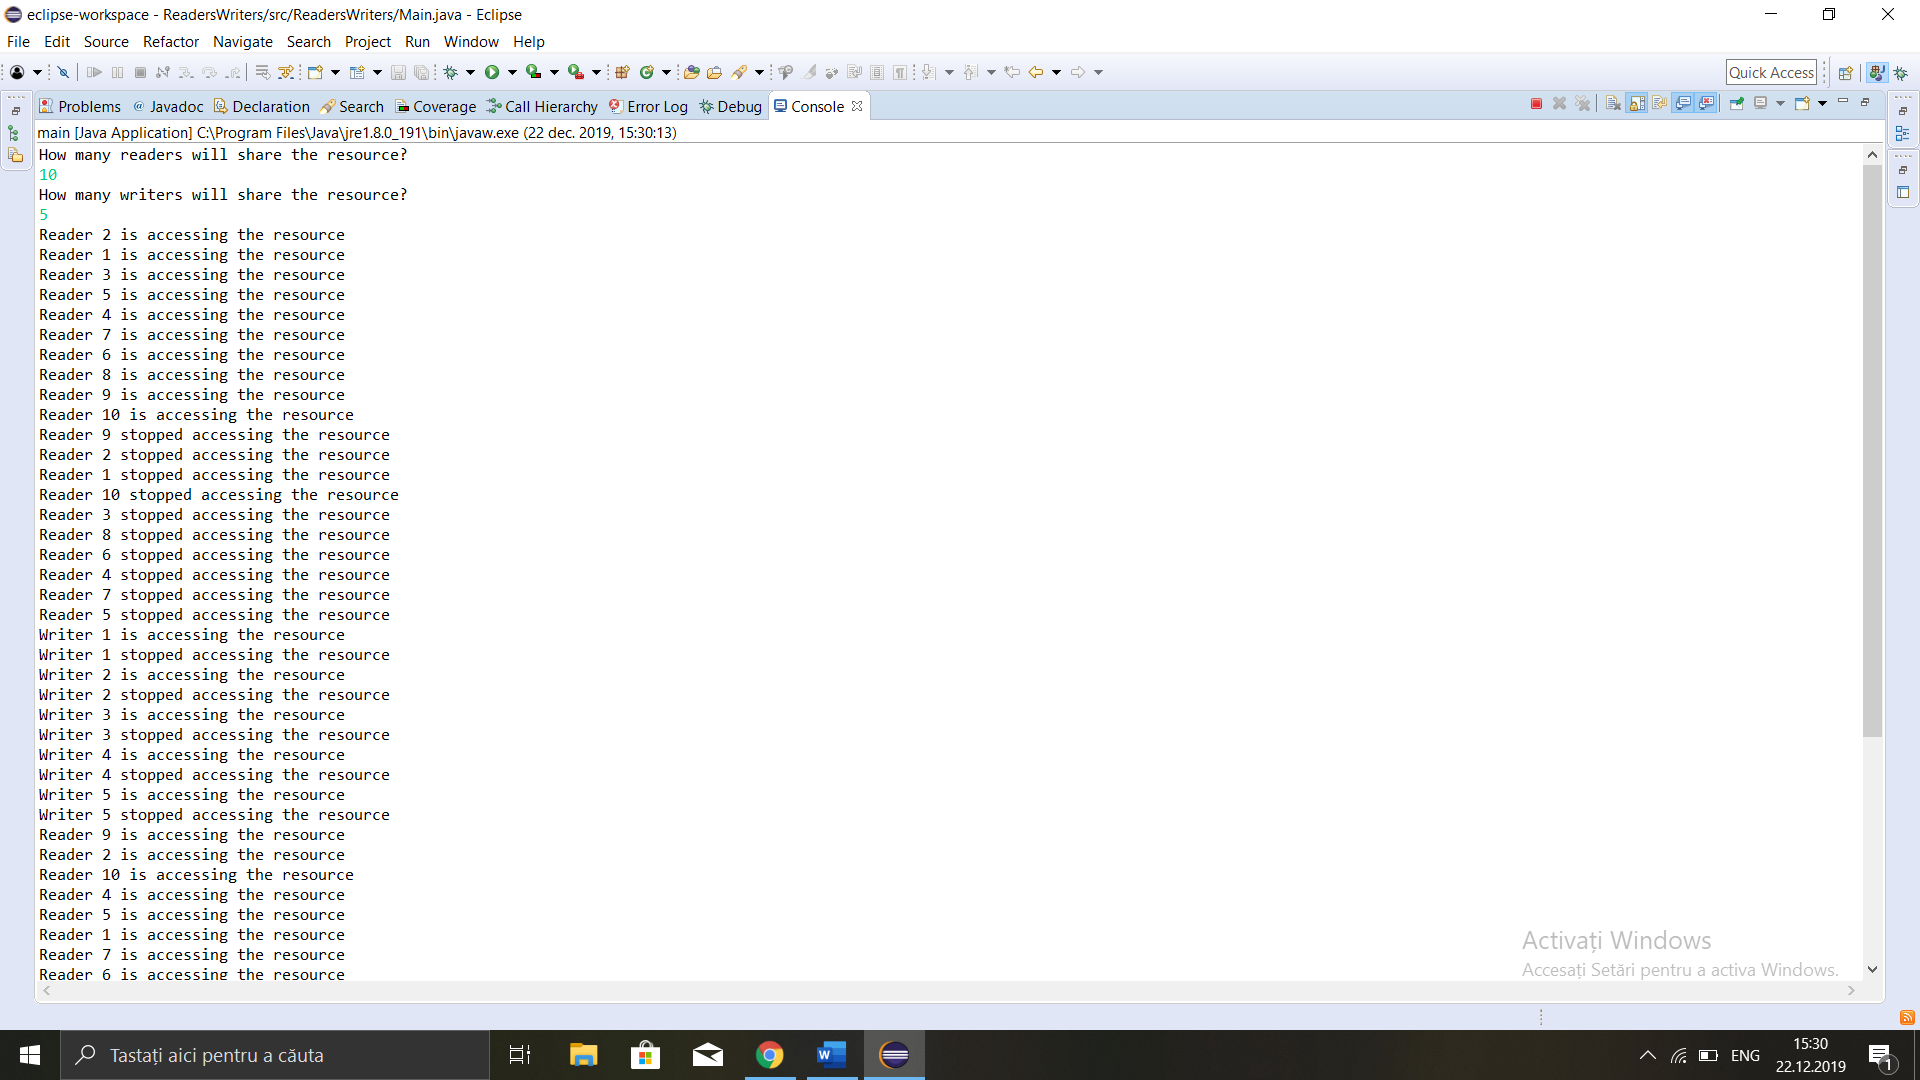
\includegraphics{RW.png}

\section{Conclusion}
\hspace{0.5 cm}
I solved the problem using 3 semaphores: resourceAccess (control acces to resource), readCountAccess (control acces to reader count), serviceQueue (control acces to the queue for read or write). In this way, deadlock and starvation were avoided.
\end{document}
